\subsubsection{Implementazione dell'AST}
L'output della fase di parsing è un oggetto di tipo \texttt{FileRepresentation}. Esso 
è sostanzialmente la radice dell'AST relativo ad un singolo file sorgente, ed è 
composto da una lista di radici di sotto-alberi corrispondenti alle definizioni contenute 
nel file. \\

\vspace{0.5cm}
\begin{lstlisting}[language=C++, frame=single]
struct FileRepresentation {

    struct Metadata {
        std::string filename;
        std::string packagename;
        std::vector<std::string> imports;
    };

    Metadata file_metadata;
    std::vector<TypeDefinition> type_defs;
    std::vector<FunctionDefinition> func_defs;
};
\end{lstlisting}
\vspace{0.5cm}

La classe \texttt{TypeDefinition} rappresenta una definizione di tipo, ed è \textit{super-tipo}
di tutti nodi dell'AST che rappresentano definizioni di tipo. \\

Si tenga presente che non necessariamente essere super tipo in C++ significa essere esteso 
tramite ereditarietà. Nello specifico, per le definizioni di tipo, la classe 
\texttt{TypeDefinition} eredita dalla classe \texttt{std::variant}, la quale è 
sostanzialmente una union. Una \texttt{TypeDefinition} infatti è implementata 
come una union delle classi \texttt{UnionDefinition}, 
\texttt{StructDefinition} e \texttt{TypeAlias}. \\ 

Anche per le classe \texttt{TypeSignature}, \texttt{Expression} e \texttt{Statement}
si è seguita la stessa logica, ovvero si è deciso di far si che esse fossero super-tipi 
di tutti i nodi dell'AST che rappresentano rispettivamente una firma di tipo, un'espressione
o una istruzione, ma ciò non è stato ottenuto tramite ereditarietà. Per queste ultime si è 
scelto di procedere all'implementazione ispirandosi ad un design pattern proprio di 
C++, ovvero il patter \textit{Type-Erasure}. \\

Tale design pattern è un wrapper su di una gerarchia classica ad oggetti basata su ereditarietà,
ma che espone una API senza puntatori, e quindi molto più comoda da usare. \\

Si è però deviati dall'implementazione classica di tale pattern, in quanto si è scelto di
conservare traccia del tipo sottostante per poter all'occorrenza verificare il tipo 
concreto dell'oggetto prima di procedere ad un cast. \\

Per tutto il resto della trattazione, si userà il termine \textit{super-tipo} con l'accezione 
appena descritta, ovvero si dirà che se oggetti di tipo \texttt{T} sono assegnabili 
ad oggetti di tipo \texttt{U}, allora \texttt{T} è un super-tipo di \texttt{U}. \\

Alla luce di tale considerazione, si può procedere all'analisi delle classi che
compongono l'AST illustrandone gli UML class diagram. Anche negli UML class diagram, 
la freccia che tipicamente indica l'ereditarietà sarà usata con l'accezione appena
descritta. \\

Di seguito segue l'UML class diagram relativo alle classi che modellano 
le espressioni in forma di AST. Si tenga presente che anche la repository
basata su ANTLR utilizza la medesima rappresentazione, e si utilizza il visitor 
autogenerato da ANTLR per navigare la rappresentazione di ANTLR e tradurla opportunamente.

\begin{figure}[H]
    \centering
        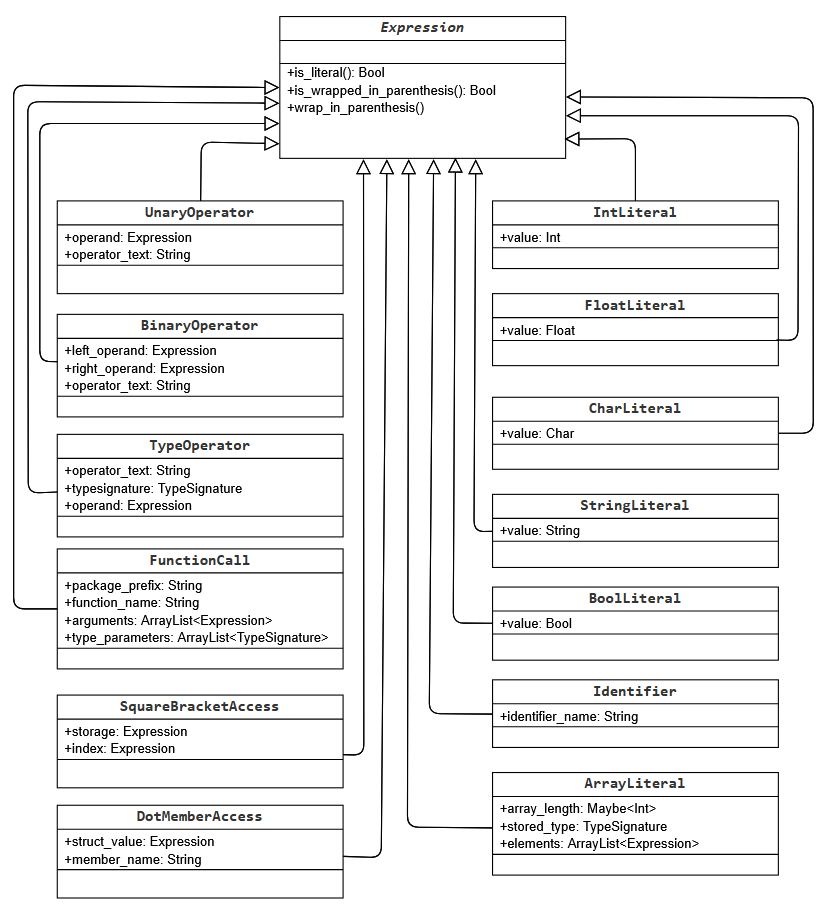
\includegraphics[width=1\textwidth]{../../Assets/AstExpr.png}
    \caption{UML class diagram dei nodi dell'AST che rappresentano espressioni}
\end{figure}

\newpage

Di seguito segue l'UML class diagram relativo alle classi che modellano 
gli statement in forma di AST. Così come già detto, anche la repository
basata su ANTLR utilizza la medesima rappresentazione, e si utilizza il visitor
autogenerato da ANTLR per navigare la rappresentazione di ANTLR e tradurla opportunamente.

\begin{figure}[H]
    \centering
        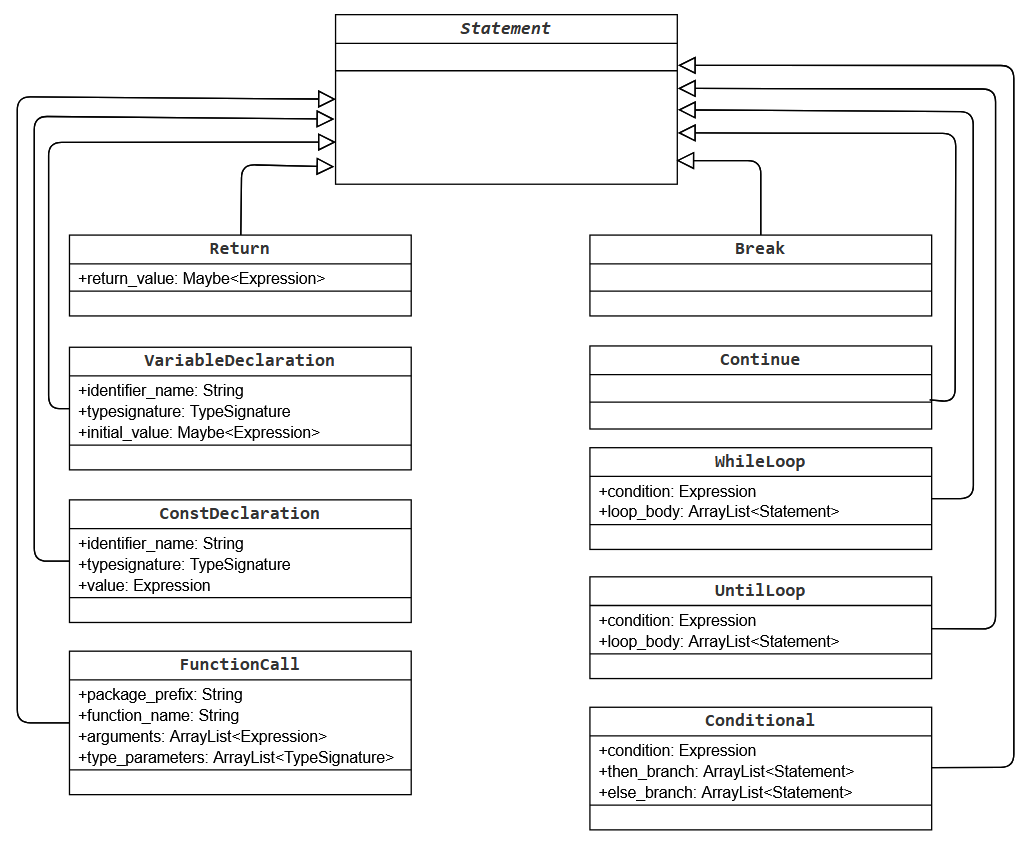
\includegraphics[width=1\textwidth]{../../Assets/StatementAST.png}
    \caption{UML class diagram dei nodi dell'AST che rappresentano statement}
\end{figure}

Si può osservare come la classe \texttt{FunctionCall} sia un sottotipo di \texttt{Expression}
e di \texttt{Statement}. Questo è dovuto al fatto che una chiamata di funzione può essere
usata sia come espressione, se restituisce un valore, sia come statement, in caso contrario. \\

Si ricordi infatti che in C++ esiste l'ereditarietà multipla, e quindi è possibile che un
una classe abbia più di un super-tipo anche nei casi in cui si usa l'eredita.

\newpage

Di seguito segue l'UML class diagram relativo alle classi che modellano type-signatures e 
definizioni di tipo in forma di AST. Così come già detto, anche la repository
basata su ANTLR utilizza la medesima rappresentazione, e si utilizza il visitor
autogenerato da ANTLR per navigare la rappresentazione di ANTLR e tradurla opportunamente.

\begin{figure}[H]
    \centering
        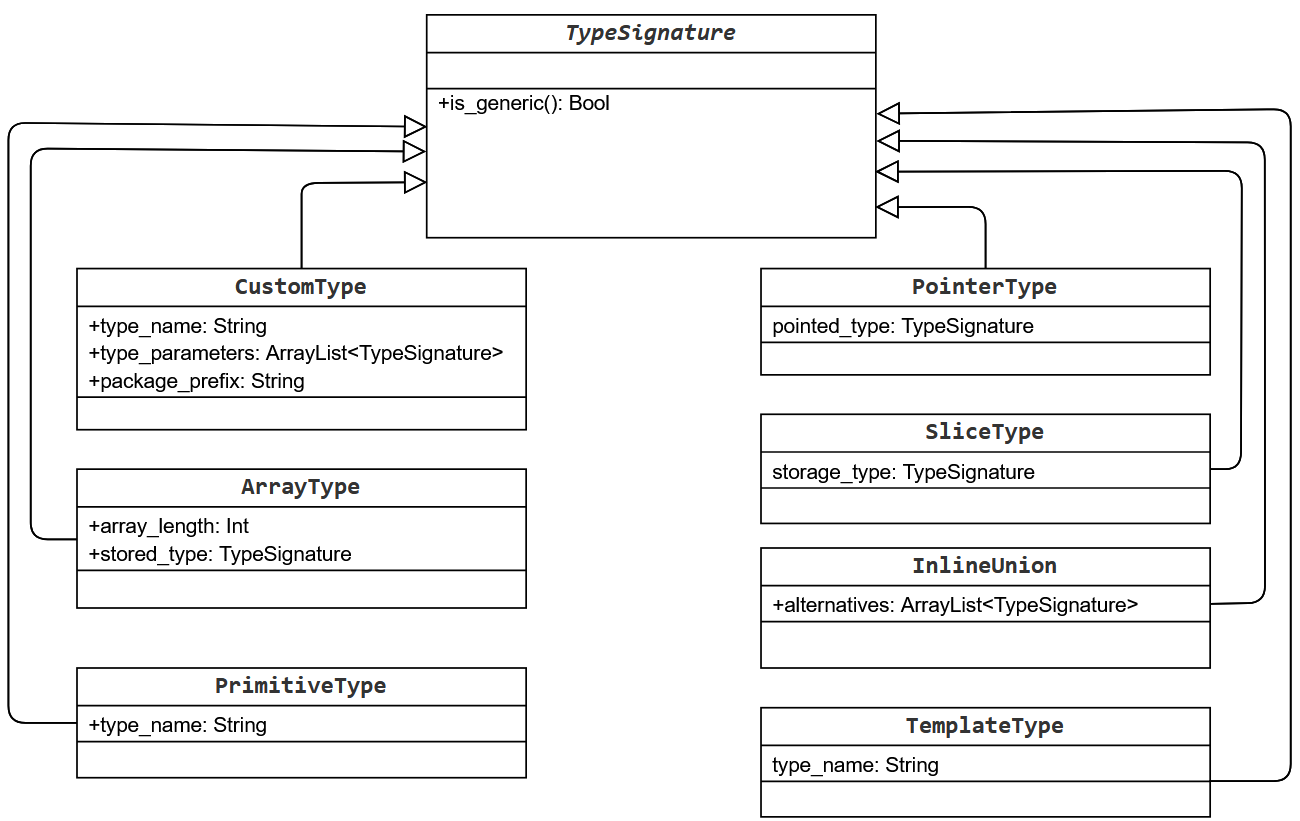
\includegraphics[width=0.9\textwidth]{../../Assets/TypeSignatureAST.png}
        \vspace{0.5cm}
        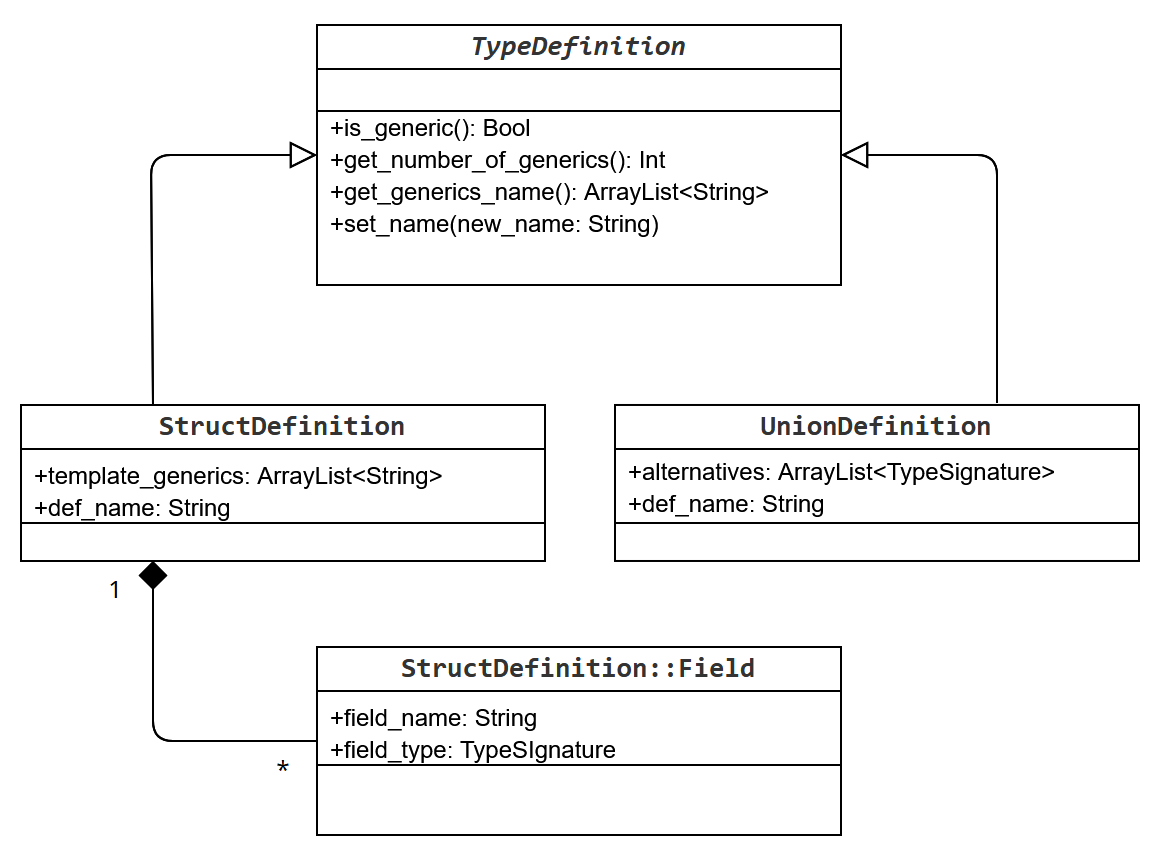
\includegraphics[width=0.7\textwidth]{../../Assets/TypeDefAST.png}
    \caption{
        \centering
        UML class diagram dei nodi dell'AST che rappresentano le type-signature
        e le definizioni di tipo
    }
\end{figure}
